
\documentclass[12pt,fleqn]{article}  
\usepackage{amsmath}
\usepackage{amssymb}
\usepackage{graphics}
\usepackage{pgfplots}

\pagestyle{empty}

\unitlength 1cm
\textheight 22cm
\textwidth 17cm
\oddsidemargin -0.5cm
\evensidemargin -0.5cm
\topmargin -1.5cm
\topskip 0cm
\headheight 0.5cm
\headsep 1cm
\marginparwidth 1.2cm

\begin{document}

\begin{center}
	\textbf{Math 2B Worksheet: 5.2 The Definite Integral}
\end{center}

\emph{Write your names and Student ID numbers at the top of the page}


\begin{enumerate}
\item Evaluate the integral using right endpoints and the definition of the integral.
\[\int_2^5(4-2x)\;dx\]
%$\int_{-2}^0(x^2+x)\;dx$

\vspace{3in}

\item Interpret the limit as a definite integral over the given interval. (Do not evaluate.)
\[\displaystyle\lim_{n\to\infty}\sum_{i=1}^nx_i\sqrt{1+x_i^3}\Delta x,\qquad [2,5]\]

% \vspace{.25in}
% (b)$\displaystyle\lim_{n\to\infty}\sum_{i=1}^n\frac{e^{x_i}}{1+x_i}\Delta x,\;[0,1]$.\\

\newpage

\item Use the graph of $g(x)$ below to evaluate the following integrals by interpreting it in terms of areas.  Note that $g$ is composed of 2 linear functions and a semi-circle.

	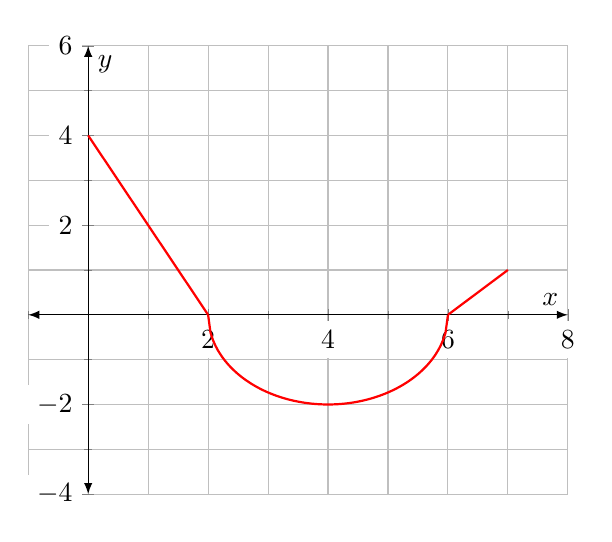
\begin{tikzpicture}
	\begin{axis}[
	 xmin=-1,xmax=8,
	ymin=-4,ymax=6,
	grid=both,
	%%grid style={line width=.1pt, draw=gray!10},
	%%major grid style={line width=.2pt,draw=gray!50},
	axis lines=middle,
	minor tick num=1,
	%%enlargelimits={abs=0.5},
	axis line style={latex-latex},
	ticklabel style={fill=white},
	xlabel=$x$,
	ylabel=$y$,	
	]
	
	\addplot [domain=0:2, mark=none,draw=red,thick] {4-2*x};
	
	\addplot [domain=2:6,samples=100, mark=none,draw=red,thick] {-sqrt(4-(x-4)^2)};
	
	\addplot [domain=6:7, mark=none,draw=red,thick] {x-6};
	
	\end{axis}
	\end{tikzpicture}
\begin{enumerate}
  \item $\displaystyle \int_0^2g(x)\;dx$\\[100pt]
  \item $\displaystyle \int_2^6g(x)\;dx$\\[100pt]
  \item $\displaystyle \int_0^7g(x)\;dx$
  \end{enumerate}
  
\end{enumerate}
\end{document}